\label{Intro.}
Water, being ``at the centre of the planetary drama of the Anthropocene'' \cite{gleesonIlluminatingwatercycle2020}, is essential not only for earth system processes but also in supporting the economic development and human well-being.
Human activities stemming from our reliance on the water have profoundly modified the natural water cycle, resulting in rivers dominated by a hybrid of social and natural tendencies
\cite{gleesonIlluminatingwatercycle2020,sivapalanSociohydrologynewscience2012,qinTheoreticalframeworkdualistic2014,abbottwatercycleAnthropocene2019,leviaHomogenizationterrestrialwater2020}.
Facing this transition, many big river basins worldwide (which are hot spots of civilization and economic growth) are urgently in need of successful water governance for sustainability
\cite{bestAnthropogenicstressesworld2019,falkenmarkUnderstandingwaterresilience2019,dibaldassarreSociohydrologyScientificChallenges2019}.
As an integral part of a proposed earth system governance framework, water governance requires a deep understanding of changes in the complex relationships between humans and water
\cite{dibaldassarreSociohydrologyScientificChallenges2019,biermannNavigatingAnthropoceneImproving2012,steffenemergenceevolutionEarth2020}.

Governance is essentially about ``who gets what, when and how''. Specifically, water governance refers to the political, social, economic, and administrative systems that influence the use and management of water %! citation.
For water resources in populated areas, missing governance means missing sustainability, and a first important step in understanding transitions toward successful water governance is identifying the different regimes.
\cite{undpwatergovernancefacilityWaterGovernanceIssue}.
Corresponding to ``who gets what, when and how'', the United Nations Development Programme (UNDP) suggests three key dimensions of water use are decided by the water governance directly: ``When and what water to use?'' (stress), ``How water provides different services to well-beings?'' (purpose), and ``Who can use water equally and efficiently?'' (allocation)
\cite{undpwatergovernancefacilityWaterGovernanceIssue, mariajacobsonUserguideassessing2013, kjellenWatergovernanceperspective2015}.

As a temporary stable state in structure, function, and dominant controls, a specific regime of water governance maintains by concreted intertwines within human-water systems (such as management, institutions, and exploitations)
\cite{carpenterEarlyWarningsRegime2011}.
However, large and persistent changes in key properties may lead to a loss of systematical stability, potentially resulting in a regime shift with impacts on system outcomes and widespread cascading effects
\cite{rochaCascadingregimeshifts2018, gregrCascadingsocialecologicalcosts2020}.
Therefore, as both signals and consequences of substantive changes in human-water systems, regime shifts align with changing three key dimensions of water governance (stress, purpose, and allocation), sometimes leading to new challenges in sustainability %! UNDP year
\cite{undpwatergovernancefacilityWaterGovernanceIssue, mariajacobsonUserguideassessing2013, kjellenWatergovernanceperspective2015}.
First, water stress depends not only on climate (with increasing scarcity and uncertainty in many regions) but also on the increasingly insatiable demands from economic activities such as irrigation and industry; water storage can resolve some but not all of these issues
\cite{greveGlobalassessmentwater2018,wadaHumanwaterinterface2017,qinFlexibilityintensityglobal2019}.
Second, the purpose of how water services human well-being is to consider trade-offs between consumptive uses (e.g., drinking and food production) and non-consumptive uses (e.g., energy production)
\cite{liuWaterscarcityassessments2017,florkeWatercompetitioncities2018,kleemannQuantifyinginterregionalflows2020}.
Third, the allocation of water across the whole basin is influenced not only by regionally socio-economic and environmental context but also by systematically regulating resources
\cite{roobavannanRoleSectoralTransformation2017,speedBasinwaterallocation2013}.
Despite regime shifts in water governance related to substantive changes in any of the three dimensions, separately considering their intertwines within human-water systems can lead to holistic failure in governing water.
The lack of a comprehensive but straightforward approach to identifying changes in water governance regimes challenges sustainability, and filling this gap can well align human and water systems (Figure~\ref{fig:framework}).

As an informative example, we focus on the Yellow River Basin (YRB, see \textit{Appendix} Methods S1 and Figure S1 for details), the fifth-largest river in the world.
With drastically anthropogenic intervention, the YRB experienced the most intense water governance challenges in China, leading to long-standing sustainability barriers.
Since the 1960s, the implementation of conservation measures, regulation reservoirs, and levee constructions have contained the issues caused by high-sediment loads
\cite{wangReducedsedimenttransport2016,wuEvolutioneffectssocialecological2020}.
However, water over-use has led to depletions of the over-burdened river, creating new challenges and new governance practices, including water use regulation and water transfer across basins
\cite{xiaDevelopmentWaterAllocation2012}.
Today, it is still impossible to completely solve water stress, trade-offs between ecosystem services, or lopsided development in different regions in the YRB; -``who gets water, when and how‘’ is still an open question for sustainable water governance
\cite{wangYellowRiverwater2019,wohlfartSocialecologicalchallengesYellow2016}.
However, confronting governance challenges induced by environmental, economic, social, and political factors, numerous governance practices have led the YRB to be among the most drastically-governing large river basins worldwide
Identifying regime shifts in water governance within the YRB can thus provide crucial insights into rapidly-changing big river basins and how governance may respond to meeting challenges to their sustainability.

% 这里我们整合了三个方向,提出了描绘流域人水关系的指数
Here, we use the three core dimensions (stress, purpose and allocation) and corresponding indicators of water governance to develop an Integrated Water Governance Index (IWGI) that can detect and describe changes in water governance at a basin-scale (see Figure~\ref{fig:framework} and methods).
% 使用案例研究
Then, by applying the index to a typical rapid-changing big river basin (the YRB), we show how to analyze the complicated regimes of water governance and their leading causes in a comprehensive but straightforward way.
% 最后总结出一般性框架
Finally, we propose a general regime transition schema as a practical guideline for a coordinated approach to exploring the challenges faced by big river basin governance.

\begin{figure*}%[htbp]

%! I don't know that fig.1 adds much, the explanatory text to the figure is the key.
	\centering
	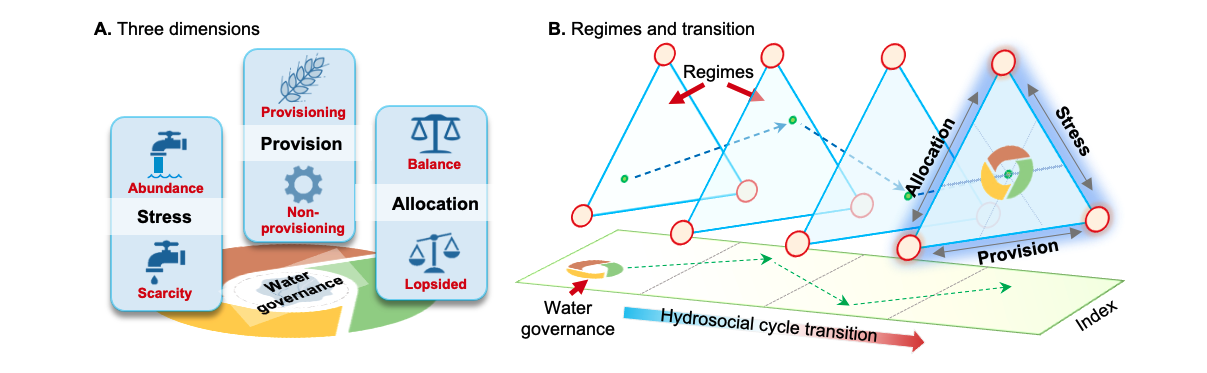
\includegraphics[width=0.9\textwidth]{main/framework.png}
	\caption{
		A framework for identifying the water governance regimes and transitions of a hydrosocial cycle.
		\textbf{A:} water governance has three key dimensions (stress, purpose and allocation), each of which has two potential directions (denoted in red) when changing: (1) ``stress'' of water shifts between scarcity and abundance; (2) ``purpose'' of water is weighted between consumptive services or non-consumptive uses; (3) ``allocation'' changes between balanced or lopsided.
		\textbf{B:} along a transition of hydrosocial water cycle, water governance shifts in line with the three dimensions. By combining corresponding indicators, an abrupt change of the IWGI thus indicates a regime shift in water governance.
		% \cite{steffenTrajectoriesEarthSystem2018,abbottwatercycleAnthropocene2019,leviaHomogenizationterrestrialwater2020}.
	}
	\label{fig:framework}
\end{figure*}
